\subsection*{SỞ GD\&ĐT NINH BÌNH\\CỤM TRƯỜNG THPT SỐ 7}

\caulc
\Opensolutionfile{ans}[ans/ans-47-26-2-Cum7NB-L1-LC]
\begin{ex}%[Câu 1]%[2D4N1-4]
	Họ nguyên hàm của hàm số $f(x)=2 \cdot 3^x$ là
	\choice
	{\True $\dfrac{2 \cdot 3^x}{\ln 3}+C$}
	{$2 \cdot 3^x \ln 3+C$}
	{$\dfrac{3^x}{\ln 3}+C$}
	{$\dfrac{2 \cdot 3^{x+1}}{x+1}+C$}
	\loigiai{
		Ta có $\displaystyle\int f(x)\mathrm{\,d}x = \displaystyle\int 2 \cdot 3^x \mathrm{\,d}x = \dfrac{2 \cdot 3^x}{\ln 3}+C$.
	}
\end{ex}


\begin{ex}%[Câu 2]%[2H5N2-2]
	Trong không gian với hệ tọa độ $Oxyz$, cho đường thẳng $(d)\colon \dfrac{x-3}{4} = \dfrac{y+2}{-5} = \dfrac{z-1}{2}$. Vectơ nào sau đây là một vectơ chỉ phương của đường thẳng $(d)$?
	\choice
	{$\vec{v}_3 = (4; 5; 2)$}
	{$\vec{v}_1 = (3; -2; 1)$}
	{$\vec{v}_4 = (3; 2; 1)$}
	{\True $\vec{v}_2 = (4; -5; 2)$}
	\loigiai{
		Phương trình đường thẳng $(d)$ có dạng chính tắc $\dfrac{x-x_0}{a} = \dfrac{y-y_0}{b} = \dfrac{z-z_0}{c}$, trong đó $(a; b; c)$ là tọa độ của một vectơ chỉ phương.
		
		Từ phương trình $(d)\colon \dfrac{x-3}{4} = \dfrac{y+2}{-5} = \dfrac{z-1}{2}$, ta suy ra đường thẳng $(d)$ có một vectơ chỉ phương là $\vec{v}_2 = (4; -5; 2)$.
	}
\end{ex}

\begin{ex}%[Câu 3]%[2H2N1-2]
	Cho hình chóp $S.ABCD$ có đáy $ABCD$ là hình bình hành (xem hình dưới). Phát biểu nào sau đây là đúng?
	\begin{center}
		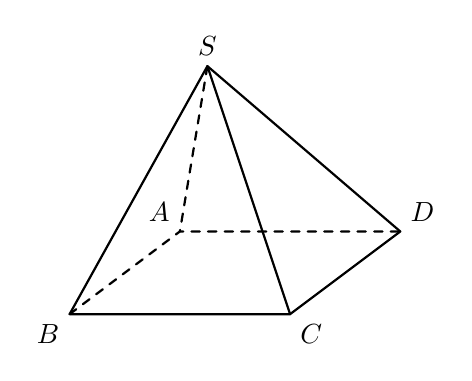
\begin{tikzpicture}[scale=0.7, thick, line join=round, line cap=round]
		% Định nghĩa toạ độ các đỉnh
		\coordinate (A) at (1,1.5);
		\coordinate (B) at (-1,0);
		\coordinate (C) at (3,0);
		\coordinate (D) at (5,1.5);
		\coordinate (S) at (1.5,4.5);
		
		% Vẽ các cạnh khuất (nét đứt)
		\draw[dashed] (B) -- (A) -- (D);
		\draw[dashed] (S) -- (A);
		
		% Vẽ các cạnh nhìn thấy (nét liền)
		\draw (S) -- (B) -- (C) -- (D) -- cycle;
		\draw (S) -- (C);
		
		% Gán nhãn các đỉnh
		\node[above] at (S) {$S$};
		\node[above left] at (A) {$A$};
		\node[below left] at (B) {$B$};
		\node[below right] at (C) {$C$};
		\node[above right] at (D) {$D$};
		\end{tikzpicture}
	\end{center}
	
	\choice
	{$\vec{SA} + \vec{SB} = \vec{SC} + \vec{SD}$}
	{\True $\vec{SA} + \vec{SC} = \vec{SB} + \vec{SD}$}
	{$\vec{AB} + \vec{AD} = \vec{CA}$}
	{$\vec{SA} - \vec{SB} = \vec{AB}$}
	
	\loigiai{
		Gọi $O$ là tâm của hình bình hành $ABCD$. Khi đó, $O$ là trung điểm của hai đường chéo $AC$ và $BD$.\\
		Áp dụng tính chất trung điểm cho các tam giác $SAC$ và $SBD$, ta có:
		\begin{itemize}
			\item $\vec{SA} + \vec{SC} = 2\vec{SO}$
			\item $\vec{SB} + \vec{SD} = 2\vec{SO}$
		\end{itemize}
		Từ đó suy ra $\vec{SA} + \vec{SC} = \vec{SB} + \vec{SD}$.\\
		Các phương án khác sai vì:
		\begin{itemize}
			\item Theo quy tắc hình bình hành ta có $\vec{AB} + \vec{AD} = \vec{AC}$ (phương án C sai).
			\item Theo quy tắc hiệu hai vectơ chung gốc ta có $\vec{SA} - \vec{SB} = \vec{BA}$ (phương án D sai).
		\end{itemize}
	}
\end{ex}
\begin{ex}%[Câu 4]%[2H2N1-1]
	Trong không gian với hệ trục tọa độ $Oxyz$, cho vectơ $\vec{u} = 2\vec{i} + 3\vec{j} - 4\vec{k}$. Tọa độ của vectơ $\vec{u}$ là
	\choice
	{\True $(2; 3; -4)$}
	{$(-2; -3; 4)$}
	{$(2; -3; 4)$}
	{$(2; 3; 4)$}
	\loigiai{
		Trong không gian $Oxyz$, một vectơ $\vec{u}$ được biểu diễn dưới dạng $\vec{u} = x\vec{i} + y\vec{j} + z\vec{k}$ sẽ có tọa độ là $(x; y; z)$.\\
		Áp dụng lý thuyết trên, với $\vec{u} = 2\vec{i} + 3\vec{j} - 4\vec{k}$, ta suy ra tọa độ của vectơ $\vec{u}$ là $(2; 3; -4)$.
	}
\end{ex}
\begin{ex}%[Câu 5]%[1D1N5-3]
	Tập nghiệm của phương trình $\sin x = 1$ là
	\choice
	{$S = \left\{ \dfrac{\pi}{2} + k\pi \mid k \in \mathbb{Z} \right\}$}
	{$S = \{ k2\pi \mid k \in \mathbb{Z} \}$}
	{\True $S = \left\{ \dfrac{\pi}{2} + k2\pi \mid k \in \mathbb{Z} \right\}$}
	{$S = \{ k\pi \mid k \in \mathbb{Z} \}$}
	
	\loigiai{
		Đây là phương trình lượng giác cơ bản: 
		$$ \sin x = 1 \Leftrightarrow x = \dfrac{\pi}{2} + k2\pi \mid k \in \mathbb{Z} $$
		Vậy tập nghiệm của phương trình là $S = \left\{ \dfrac{\pi}{2} + k2\pi \mid k \in \mathbb{Z} \right\}$.\\
		
	}
\end{ex}


\begin{ex}%[Câu 6]%[1D2N2-4]
	Cho cấp số cộng $(u_n)$ có $u_1 = 5$ và công sai $d = 4$. Giá trị của $u_6$ bằng
	\choice
	{$29$}
	{\True $25$}
	{$20$}
	{$24$}
	
	\loigiai{
		Theo công thức số hạng tổng quát của cấp số cộng, ta có:
		$$u_n = u_1 + (n-1)d$$
		Thay $n=6, u_1 = 5, d = 4$ vào công thức trên, ta được:
		$$u_6 = 5 + (6-1) \cdot 4 = 5 + 5 \cdot 4 = 5 + 20 = 25$$
		Vậy giá trị của $u_6$ là $25$.
	}
\end{ex}
\begin{ex}%[Câu 7]%[1D6N4-2]
	Nghiệm của phương trình $\log_3(2x-3)=2$ là
	\choice
	{$x=\frac{7}{2}$}
	{$x=\frac{5}{2}$}
	{\True $x=6$}
	{$x=5$}
	
	\loigiai{
		Điều kiện xác định: $2x - 3 > 0 \Leftrightarrow x > \frac{3}{2}$.\\
		Ta có: 
		$$ \log_3(2x-3) = 2 $$
		$$ \Leftrightarrow 2x - 3 = 3^2 $$
		$$ \Leftrightarrow 2x - 3 = 9 $$
		$$ \Leftrightarrow 2x = 12 $$
		$$ \Leftrightarrow x = 6 \text{ (thỏa mãn điều kiện)} $$
		Vậy phương trình có nghiệm là $x = 6$.\\
		\textbf{Chọn C.}
	}
\end{ex}

\begin{ex}%[Câu 8]%[2D1H1-2]
	Cho hàm số $y = f(x)$ có đạo hàm trên $\mathbb{R}$ và hàm số $y = f'(x)$ có đồ thị như hình sau
	\begin{center}
		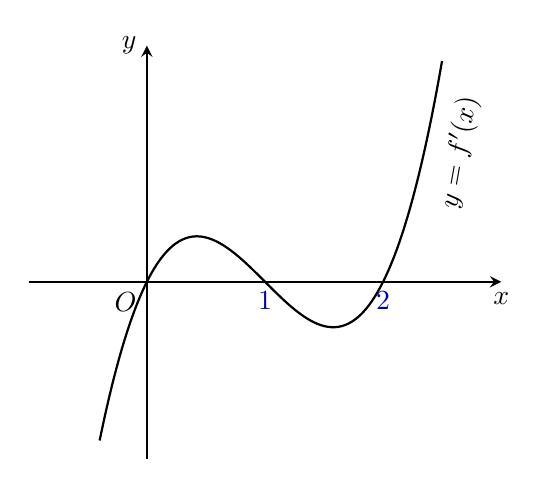
\begin{tikzpicture}[>=stealth, scale=1.5, thick]
		% Trục tọa độ
		\draw[->, color=black!70!black] (-1,0) -- (3,0) node[below] {$x$};
		\draw[->, color=black!70!black] (0,-1.5) -- (0,2) node[left] {$y$};
		\node[below left, color=black!70!black] at (0,0) {$O$};
		
		% Các điểm trên trục hoành
		\node[below, color=blue!70!black] at (1,0) {$1$};
		\node[below, color=blue!70!black] at (2,0) {$2$};
		
		% Vẽ đồ thị f'(x)
		% Dùng hàm x(x-1)(x-2) = x^3 - 3x^2 + 2x để mô phỏng dáng đồ thị
		\draw[color=black, smooth, samples=100, domain=-0.4:2.5] 
		plot (\x, {(\x)*(\x-1)*(\x-2)});
		
		\node[above right, rotate=80, color=black!70!black] at (2.75, 0.5) {$y = f'(x)$};
		%\node[below, color=blue!70!black] at (1, -1.5) {\textit{Hình 31}};
		\end{tikzpicture}
	\end{center}
	Hàm số $y = f(x)$ đồng biến trên khoảng nào trong các khoảng sau?
	\choice
	{$(-\infty ; 0)$}
	{\True $(0 ; 1)$}
	{$(0 ; 2)$}
	{$(1 ; 2)$}
	
	\loigiai{
		Hàm số $y = f(x)$ đồng biến trên các khoảng mà $f'(x) > 0$ (tức là phần đồ thị $y = f'(x)$ nằm phía trên trục hoành).\\
		Dựa vào đồ thị, ta thấy $f'(x) > 0$ khi $x \in (0; 1)$ hoặc $x \in (2; +\infty)$.\\
		Đối chiếu với các phương án, ta thấy hàm số đồng biến trên khoảng $(0; 1)$.\\
		\textbf{Chọn B.}
	}
\end{ex}

\begin{ex}%[Câu 9]%[2H5H2-3]
	Trong không gian $Oxyz$, cho hai điểm $A(1;-2;3)$ và $B(3;1;1)$. Đường thẳng $AB$ có phương trình là
	\choice
	{$\dfrac{x-1}{4}=\dfrac{y+2}{-1}=\dfrac{z-3}{4}$}
	{\True $\dfrac{x-1}{2}=\dfrac{y+2}{3}=\dfrac{z-3}{-2}$}
	{$\dfrac{x-4}{1}=\dfrac{y+1}{-2}=\dfrac{z-4}{3}$}
	{$\dfrac{x-2}{2}=\dfrac{y-3}{-2}=\dfrac{z+2}{3}$}
	\loigiai{
		Ta có $\overrightarrow{AB}(2;3;-2)$. Suy ra đường thẳng $AB$ có $1$ vectơ chỉ phương là $\overrightarrow{u}(2;3;-2)$.\\
		Mà đường thẳng $AB$ đi qua điểm $A(1;-2;3)$ nên $AB$ có phương trình chính tắc là $$\dfrac{x-1}{2}=\dfrac{y+2}{3}=\dfrac{z-3}{-2}.$$}
\end{ex}

\begin{ex}%[Câu 10]%[1H8H5-2]
	Cho hình lập phương $ABCD.A'B'C'D'$ có cạnh bằng $2a$. Khoảng cách từ điểm $C$ đến mặt phẳng $(A'BD)$ bằng
	\begin{center}
		\begin{tikzpicture}[scale=0.6, font=\footnotesize,line join=round, line cap=round, >=stealth]
		\path 
		(0,0) coordinate (A)
		++(-130:3) coordinate (B)
		++(0:4) coordinate (C)
		($(A)+(C)-(B)$) coordinate (D)
		%($(A)!1/2!(C)$) coordinate (O)
		;
		
		\foreach \i in {A,B,C,D}{
			\coordinate (\i') at ($(\i)+(0,4)$);
		}
		%\coordinate (K) at ($(A')!(A)!(O)$);
		
		\draw[blue] (A')--(B')--(C')--(D')--cycle;
		\draw[blue] (B)--(B') (C)--(C') (D)--(D')  (B)--(C)--(D);
		\draw[blue,dashed,thin] (B)--(A)--(A') (C)--(A)--(D) (A')--(B)--(D)--cycle;
		%\draw[blue,dashed,thin] (A')--(O) (A)--(K);
		
		%\pic[draw=blue,angle eccentricity=1.8,angle radius=2mm]{right angle=B--O--C};
		%\pic[draw=blue,angle eccentricity=1.8,angle radius=2mm]{right angle=A--K--O};
		
		% Đã thêm phần góc "/0" cho điểm D để vòng lặp không bị lỗi
		\foreach \i/\g in {A'/90,B'/90,C'/-140,D'/90,A/-90,B/-90,C/-90,D/0}
		\fill[blue] (\i) circle(1pt)+(\g:4mm)node[scale=1]{$\i$};
		\end{tikzpicture}
	\end{center}
	\choice
	{\True $\dfrac{2a\sqrt{3}}{3}$}
	{$\dfrac{4a\sqrt{3}}{3}$}
	{$a\sqrt{3}$}
	{$\dfrac{a\sqrt{3}}{3}$}
	\loigiai{
		\immini
		{Gọi $O = AC \cap BD$. Ta có $AC \cap (A'BD) = O$.\\
			Do $O$ là trung điểm của $AC$ nên $d(C, (A'BD)) = d(A, (A'BD))$.\\
			Vì $ABCD$ là hình vuông nên $AO \perp BD$.\\
			Mặt khác $AA' \perp (ABCD) \Rightarrow AA' \perp BD$.\\
			Suy ra $BD \perp (A'AO) \Rightarrow (A'BD) \perp (A'AO)$.\\
			Trong mặt phẳng $(A'AO)$, kẻ $AK \perp A'O$ tại $K$, ta có $AK \perp (A'BD)$.\\
			Do đó $d(A, (A'BD)) = AK$.\\
			Ta có $AA' = 2a$ và $AO = \dfrac{AC}{2} = \dfrac{2a\sqrt{2}}{2} = a\sqrt{2}$.\\
			Xét tam giác $A'AO$ vuông tại $A$ có $AK$ là đường cao:\\
			$\dfrac{1}{AK^2} = \dfrac{1}{AA'^2} + \dfrac{1}{AO^2} = \dfrac{1}{(2a)^2} + \dfrac{1}{(a\sqrt{2})^2} = \dfrac{1}{4a^2} + \dfrac{1}{2a^2} = \dfrac{3}{4a^2}$.\\
			Suy ra $AK = \dfrac{2a\sqrt{3}}{3}$.\\
			Vậy $d(C, (A'BD)) = \dfrac{2a\sqrt{3}}{3}$.}
		{\begin{tikzpicture}[scale=0.6, font=\footnotesize,line join=round, line cap=round, >=stealth]
			\path 
			(0,0) coordinate (A)
			++(-130:3) coordinate (B)
			++(0:4) coordinate (C)
			($(A)+(C)-(B)$) coordinate (D)
			($(A)!1/2!(C)$) coordinate (O)
			;
			\foreach \i in {A,B,C,D}{
				\coordinate (\i') at ($(\i)+(0,4)$);
			}
			\coordinate (K) at ($(A')!(A)!(O)$);
			
			\draw[blue] (A')--(B')--(C')--(D')--cycle;
			\draw[blue] (B)--(B') (C)--(C') (D)--(D')  (B)--(C)--(D);
			\draw[blue,dashed,thin] (B)--(A)--(A') (C)--(A)--(D) (A')--(B)--(D)--cycle;
			\draw[blue,dashed,thin] (A')--(O) (A)--(K);
			
			\pic[draw=blue,angle eccentricity=1.8,angle radius=2mm]{right angle=B--O--C};
			\pic[draw=blue,angle eccentricity=1.8,angle radius=2mm]{right angle=A--K--O};
			
			\foreach \i/\g in {A'/90,B'/90,C'/-140,D'/90,A/-90,B/-90,C/-90,D/-90,O/-90,K/30}
			\fill[blue] (\i) circle(1pt)+(\g:4mm)node[scale=1]{$\i$};
			\end{tikzpicture}}
	}
\end{ex}


\begin{ex}%[Câu 11]%[2D4H3-3]
	Cho hình phẳng $(H)$ giới hạn bởi đồ thị $y=3x-x^2$ và trục hoành. Thể tích vật thể tròn xoay sinh ra khi cho $(H)$ quay quanh trục hoành bằng
	\choice
	{$\dfrac{81}{10}$}
	{\True $\dfrac{81\pi}{10}$}
	{$\dfrac{81\pi}{5}$}
	{$\dfrac{27\pi}{10}$}
	\loigiai{
		Phương trình hoành độ giao điểm của đồ thị $y=3x-x^2$ và trục hoành là
		$$3x-x^2=0\Leftrightarrow \hoac{&x=0 \\&x=3.}$$
		Thể tích vật thể tròn xoay sinh ra khi cho $(H)$ quay quanh trục hoành là
		$$V=\pi \displaystyle\int\limits_0^3\left(3x-x^2\right)^2\mathrm{\,d}x = \pi \displaystyle\int\limits_0^3\left(9x^2-6x^3+x^4\right)\mathrm{\,d}x = \pi \left.\left(3x^3-\dfrac{3x^4}{2}+\dfrac{x^5}{5}\right)\right|_0^3 = \dfrac{81\pi}{10}.$$}
\end{ex}
\begin{ex}%[Câu 12]%[1D5H2-3]
	Một người chia thời lượng (đơn vị: giây) thực hiện các cuộc gọi điện thoại của mình trong một tuần thành sáu nhóm và lập bảng tần số ghép nhóm như sau
	\begin{center}
		\renewcommand{\arraystretch}{1.5}
		\begin{tabular}{|c|c|c|c|c|c|c|}
			\hline
			\textbf{Nhóm} & $[0;40)$ & $[40;80)$ & $[80;120)$ & $[120;160)$ & $[160;200)$ & $[200;240)$ \\
			\hline
			\textbf{Tần số} & 11 & 10 & 6 & 8 & 4 & 1 \\
			\hline
		\end{tabular}
	\end{center}
	Tứ phân vị thứ nhất $Q_1$ (đơn vị: giây) của mẫu số liệu ghép nhóm trên bằng
	\choice
	{$36$}
	{$40$}
	{\True $\dfrac{400}{11}$}
	{$\dfrac{420}{11}$}
	\loigiai{
		Cỡ mẫu là $n = 11 + 10 + 6 + 8 + 4 + 1 = 40$.\\
		Gọi $x_1, x_2, \dots, x_{40}$ là mẫu số liệu được xếp theo thứ tự không giảm.\\
		Vị trí của tứ phân vị thứ nhất là $\frac{n}{4} = \frac{40}{4} = 10$.\\
		Tần số tích lũy của nhóm đầu tiên là $11$.\\
		Vì $10 \le 11$ nên giá trị $x_{10}$ (và cả $x_{11}$) đều thuộc nhóm thứ nhất là $[0;40)$.\\
		Do đó, nhóm chứa tứ phân vị thứ nhất là nhóm $[0;40)$.\\
		Áp dụng công thức tính tứ phân vị thứ nhất cho mẫu số liệu ghép nhóm, ta có:
		$$Q_1 = 0 + \frac{10 - 0}{11} \cdot (40 - 0) = \frac{400}{11} \approx 36,36.$$
		Vậy tứ phân vị thứ nhất $Q_1$ bằng $\frac{400}{11}$.\\
		\textbf{Chọn A.}
	}
\end{ex}


\Closesolutionfile{ans}


\cauds
\Opensolutionfile{ans}[ans/ans-47-26-2-Cum7NB-L1-DS]
\begin{ex}%[2D1H3-1]
	Cho hàm số $f(x) = x^3 - 27x + 10$.
	\choiceTF
	{\True Hàm số đã cho có đạo hàm là $f'(x) = 3x^2 - 27$}
	{Phương trình $f'(x) = 0$ có tập nghiệm là $S = \{3\}$}
	{$f(3) = 44$}
	{Giá trị lớn nhất của hàm số $f(x)$ trên đoạn $[-4;4]$ bằng $54$}
	
	\loigiai{
		\begin{itemchoice}
			\itemch Ta có $f'(x) = (x^3 - 27x + 10)' = 3x^2 - 27$. Vậy mệnh đề \textbf{Đúng}.
			
			\itemch Phương trình $f'(x) = 0 \Leftrightarrow 3x^2 - 27 = 0 \Leftrightarrow x^2 = 9 \Leftrightarrow x = \pm 3$.\\
			Tập nghiệm của phương trình là $S = \{-3; 3\}$. Vậy mệnh đề \textbf{Sai}.
			
			\itemch Thay $x = 3$ vào hàm số, ta có: $f(3) = 3^3 - 27 \cdot 3 + 10 = 27 - 81 + 10 = -44$.\\
			Vậy mệnh đề \textbf{Sai}.
			
			\itemch Xét hàm số $f(x)$ trên đoạn $[-4; 4]$.\\
			Ta có $f'(x) = 0 \Leftrightarrow x = \pm 3$ (cả hai nghiệm đều thuộc đoạn $[-4; 4]$).\\
			Tính các giá trị:
			\begin{itemize}
				\item $f(-4) = (-4)^3 - 27(-4) + 10 = -64 + 108 + 10 = 54$.
				\item $f(-3) = (-3)^3 - 27(-3) + 10 = -27 + 81 + 10 = 64$.
				\item $f(3) = 3^3 - 27(3) + 10 = -44$.
				\item $f(4) = 4^3 - 27(4) + 10 = 64 - 108 + 10 = -34$.
			\end{itemize}
			So sánh các giá trị trên, ta thấy $\max\limits_{[-4; 4]} f(x) = 64$ khi $x = -3$.\\
			Vậy mệnh đề \textbf{Sai}.
		\end{itemchoice}
	}
\end{ex}




\begin{ex}%[2D4V1-6]
	Một mẫu đồng vị phóng xạ (ví dụ: Iodine-131 được sử dụng trong y tế) có khối lượng ban đầu là $800 \text{ mg}$. Sau $5$ ngày, khối lượng của mẫu chất này phân rã và chỉ còn lại $400 \text{ mg}$. Gọi $m(t)$ là khối lượng của mẫu chất phóng xạ tại thời điểm $t$ (ngày). Biết rằng tốc độ phân rã của mẫu chất tỉ lệ thuận với khối lượng hiện có của nó, tức là $m'(t) = k \cdot m(t)$, với $k$ là hằng số khác $0$ và $m(t)>0$ với $t\geq 0$.
	\choiceTF
	{\True Hằng số tốc độ phân rã của mẫu chất là $k = -\frac{1}{5}\ln 2$}
	{\True Sau $15$ ngày kể từ thời điểm ban đầu, khối lượng mẫu chất còn lại là $100 \text{ mg}$}
	{Khối lượng của mẫu chất phóng xạ được tính bởi công thức $m(t) = 400e^{kt}$ với $t \ge 0$}
	{Để khối lượng mẫu chất phân rã chỉ còn $50 \text{ mg}$, cần đúng $10$ ngày kể từ thời điểm ban đầu}
	
	\loigiai{
		Từ phương trình vi phân $m'(t) = k \cdot m(t)$, ta có nghiệm tổng quát mô tả khối lượng mẫu chất là $m(t) = C_0 \cdot e^{kt}$.\\
		Tại thời điểm ban đầu $t = 0$, khối lượng mẫu là $m(0) = 800 \Rightarrow C_0 \cdot e^0 = 800 \Rightarrow C_0 = 800$.\\
		Do đó, hàm số biểu diễn khối lượng là $m(t) = 800e^{kt}$.\\
		Sau $5$ ngày ($t = 5$), khối lượng còn lại là $m(5) = 400$.
		
		\begin{itemchoice}
			\itemch Ta có $m(5) = 400 \Leftrightarrow 800e^{5k} = 400 \Leftrightarrow e^{5k} = \frac{1}{2} \Leftrightarrow 5k = \ln\left(\frac{1}{2}\right) \Leftrightarrow k = -\frac{1}{5}\ln 2$.\\
			Khẳng định đề bài hoàn toàn chính xác, do đó mệnh đề \textbf{Đúng}.
			
			\itemch Tại thời điểm $t = 15$ ngày, khối lượng mẫu chất còn lại là:\\
			$m(15) = 800e^{15k} = 800 \cdot \left(e^{5k}\right)^3 = 800 \cdot \left(\frac{1}{2}\right)^3 = 800 \cdot \frac{1}{8} = 100 \text{ (mg)}$.\\
			Khẳng định đề bài là $100 \text{ mg}$, do đó mệnh đề \textbf{Đúng}.
			
			\itemch Dựa vào chứng minh ban đầu, do $m(0) = 800$ nên biểu thức phải là $m(t) = 800e^{kt}$ với mọi $t \ge 0$.\\
			Khẳng định đề bài ghi là $400e^{kt}$, vậy mệnh đề \textbf{Sai}.
			
			\itemch Để khối lượng mẫu chất giảm xuống còn $50 \text{ mg}$, ta giải phương trình:
			$$m(t) = 50 \Leftrightarrow 800e^{kt} = 50 \Leftrightarrow e^{kt} = \frac{1}{16}.$$
			Mặt khác, $e^{kt} = e^{\left(-\frac{1}{5}\ln 2\right)t} = \left(e^{-\ln 2}\right)^{\frac{t}{5}} = \left(\frac{1}{2}\right)^{\frac{t}{5}}$.\\
			Suy ra: $\left(\frac{1}{2}\right)^{\frac{t}{5}} = \frac{1}{16} = \left(\frac{1}{2}\right)^4 \Leftrightarrow \frac{t}{5} = 4 \Leftrightarrow t = 20 \text{ (ngày)}$.\\
			Khẳng định đề bài ghi là cần $10$ ngày, vậy mệnh đề \textbf{Sai}.
		\end{itemchoice}
	}
\end{ex}


\begin{ex}%[2D6V2-3]
	Một bệnh viện sử dụng hai phác đồ điều trị $A$ và $B$ cho một loại bệnh. Có $60\%$ bệnh nhân được chỉ định điều trị bằng phác đồ $A$ và $40\%$ bệnh nhân điều trị bằng phác đồ $B$. Tỉ lệ bệnh nhân gặp tác dụng phụ khi sử dụng phác đồ $A$ và phác đồ $B$ lần lượt là $5\%$ và $3\%$. Chọn ngẫu nhiên một bệnh nhân đang điều trị căn bệnh này tại bệnh viện.
	\choiceTF
	{Nếu bệnh nhân được chọn đang điều trị bằng phác đồ $A$ thì xác suất để người đó không gặp tác dụng phụ là $0{,}97$}
	{\True Xác suất để bệnh nhân được chọn gặp tác dụng phụ và đang điều trị bằng phác đồ $A$ là $0{,}03$}
	{\True Xác suất để bệnh nhân được chọn gặp tác dụng phụ là $0{,}042$}
	{Nếu bệnh nhân được chọn gặp tác dụng phụ thì xác suất để người đó được điều trị bằng phác đồ $A$ là $\dfrac{6}{7}$}
	\loigiai
	{Gọi $A$, $B$ lần lượt là biến cố chọn được bệnh nhân điều trị bằng phác đồ $A$, $B$.\\
		Ta có $\mathrm{P}(A)=0{,}6$; $\mathrm{P}(B)=0{,}4$.\\
		Gọi $C$ là biến cố chọn được bệnh nhân gặp tác dụng phụ.\\
		Tỉ lệ gặp tác dụng phụ của phác đồ $A$ là $5 \% \Rightarrow \mathrm{P}(C \mid A)=0{,}05$.\\
		Tỉ lệ gặp tác dụng phụ của phác đồ $B$ là $3 \% \Rightarrow \mathrm{P}(C \mid B)=0{,}03$.
		\begin{itemchoice}
			\itemch Nếu bệnh nhân được chọn điều trị bằng phác đồ $A$ thì xác suất để người đó không gặp tác dụng phụ là $\mathrm{P}(\overline{C}\left| A\right.)=1-\mathrm{P}(C\left| A\right.)=1-0{,}05=0{,}95$. Do đó phát biểu này \textbf{Sai}.
			\itemch Xác suất để bệnh nhân được chọn gặp tác dụng phụ và điều trị bằng phác đồ $A$ là $\mathrm{P}(A\cap C)=\mathrm{P}(A)\cdot \mathrm{P}(C\left| A\right.)=0{,}6\cdot 0{,}05=0{,}03$. Do đó phát biểu này \textbf{Đúng}.
			\itemch Xác suất để bệnh nhân được chọn gặp tác dụng phụ là tổng xác suất gặp tác dụng phụ từ nhóm dùng phác đồ $A$ và nhóm dùng phác đồ $B$ là
			$$\mathrm{P}(C)=\mathrm{P}(A)\cdot \mathrm{P}(C\left| A\right.)+\mathrm{P}(B)\cdot \mathrm{P}(C\left| B\right.)=0{,}6\cdot 0{,}05+0{,}4\cdot 0{,}03=0{,}042.$$
			Do đó phát biểu này \textbf{Đúng}.
			\itemch Nếu bệnh nhân được chọn gặp tác dụng phụ thì xác suất để người đó điều trị bằng phác đồ $A$ là $$\mathrm{P}(A\left| C\right.)=\dfrac{\mathrm{P}(A\cap C)}{\mathrm{P}(C)}=\dfrac{0{,}03}{0{,}042}=\dfrac{5}{7}.$$
			Do đó phát biểu này \textbf{Sai}.
		\end{itemchoice}
	}
\end{ex}

\begin{ex}%[2H2H2-6]
	Trong không gian với hệ trục tọa độ $Oxyz$, đơn vị trên mỗi trục toạ độ là mét và mặt phẳng $(Oxy)$ trùng với mặt đất. Một cabin cáp treo xuất phát từ điểm $A(-50;10;20)$ và chuyển động thẳng đều đến điểm $B(1550;-190;820)$ với tốc độ là $6$ (m/s). Một camera giám sát an toàn được đặt tại vị trí $C(754;-86;413)$.
	\choiceTF
	{Vectơ $\overrightarrow{u}(8;1;4)$ là một vectơ chỉ phương của quỹ đạo di chuyển của cabin}
	{\True Thời gian cabin cáp treo đi từ $A$ đến $B$ là $5$ phút}
	{\True Sau khi di chuyển từ $A$ được $1$ phút, cabin cáp treo cách mặt đất $180$ mét}
	{\True Khoảng cách ngắn nhất từ cabin đến camera giám sát an toàn là $9$ mét và đạt được sau $150$ giây kể từ lúc xuất phát}
	\loigiai
	{
		\begin{itemchoice}
			\itemch Ta có $\overrightarrow{AB}=(1600;-200;800)=200(8;-1;4)$. Quỹ đạo chuyển động là đường thẳng $AB$ nên nhận $\overrightarrow{u}(8;-1;4)$ làm vectơ chỉ phương chứ không phải $(8;1;4)$.
			\itemch Ta có $\left| \overrightarrow{AB}\right|=\sqrt{1600^2+(-200)^2+800^2}=1800$ (mét). \\
			Thời gian cabin di chuyển hết hành trình là $t=\dfrac{1800}{6}=300$ (giây).\\
			Đổi $300$ giây $= 5$ phút. Vậy phát biểu này đúng.
			\itemch Quãng đường cabin di chuyển được sau $1$ phút ($60$ giây) là $S = 6 \cdot 60 = 360$ (mét).\\
			Gọi $K(x;y;z)$ là vị trí của cabin sau $1$ phút. Ta có $\overrightarrow{AK} = \dfrac{360}{1800}\overrightarrow{AB} = \dfrac{1}{5}\overrightarrow{AB}$.\\
			Suy ra cao độ của điểm $K$ là $z_K - z_A = \dfrac{1}{5}(z_B - z_A) \Rightarrow z_K - 20 = \dfrac{1}{5} \cdot 800 \Rightarrow z_K = 180$.\\
			Do mặt phẳng $(Oxy)$ trùng với mặt đất nên khoảng cách từ cabin đến mặt đất chính là $|z_K|=180$ mét. Phát biểu này đúng.
			\itemch Đường thẳng $AB$ đi qua $A(-50; 10; 20)$ và có vectơ chỉ phương $\overrightarrow{u}(8; -1; 4)$ nên có phương trình tham số: $\begin{cases} x = -50 + 8s \\ y = 10 - s \\ z = 20 + 4s \end{cases}$.\\
			Giả sử $H$ là vị trí cabin trên cáp treo sao cho khoảng cách từ cabin đến camera $C$ là ngắn nhất. Khi đó $H$ là hình chiếu vuông góc của $C$ trên đường thẳng $AB$.\\
			Suy ra $H(-50+8s; 10-s; 20+4s) \Rightarrow \overrightarrow{CH} = (8s - 804; -s + 96; 4s - 393)$.\\
			Ta có $\overrightarrow{CH} \perp \overrightarrow{u} \Leftrightarrow 8(8s - 804) - 1(-s + 96) + 4(4s - 393) = 0 \Leftrightarrow 81s - 8100 = 0 \Leftrightarrow s = 100$.\\
			Với $s=100$, ta có $\overrightarrow{CH} = (-4; -4; 7)$. Khoảng cách ngắn nhất là $CH = \sqrt{(-4)^2 + (-4)^2 + 7^2} = 9$ (mét).\\
			Tọa độ $H(750; -90; 420)$. Quãng đường cabin đã đi là $AH = \sqrt{800^2 + (-100)^2 + 400^2} = 900$ (mét).\\
			Thời gian để cabin đến được vị trí gần camera nhất là $t_H = \dfrac{900}{6} = 150$ (giây). Phát biểu này đúng.
		\end{itemchoice}
	}
\end{ex}
\Closesolutionfile{ans}

\caukq
\Opensolutionfile{ans}[ans/ans-47-26-2-Cum7NB-L1-KQ]
\begin{ex}%[2D6C1-4]
	Có hai túi A và B, mỗi túi chứa $3$ quả bóng được ghi các số $1$, $2$, $3$. Một người chơi rút ngẫu nhiên một quả bóng từ túi A, và người kia rút ngẫu nhiên một quả bóng từ túi B, ghi lại số trên bóng rồi trả lại túi của mình. Thí nghiệm này được lặp lại hai lần. Khi tổng hai số của người rút từ túi A lớn hơn tổng hai số của người rút từ túi B, xác suất để tổng hai số của người rút từ túi A là $5$ là $\dfrac{q}{p}$ (với $p, q$ là các số nguyên tố cùng nhau). Tính giá trị của biểu thức $p + q$.
	\shortans{$43$}
	\loigiai{
		Gọi $X$ là tổng các số trên $2$ quả bóng rút ra từ túi A sau hai lần rút (có hoàn lại).
		
		Gọi $Y$ là tổng các số trên $2$ quả bóng rút ra từ túi B sau hai lần rút (có hoàn lại).
		
		Vì hai túi A và B có cấu trúc như nhau và cách thức rút giống nhau nên $X, Y$ độc lập và có cùng một bảng phân bố xác suất.
		
		Mỗi lần rút từ một túi, số kết quả có thể xảy ra là $3$. Sau $2$ lần rút, số phần tử không gian mẫu cho mỗi người là $n(\Omega_X) = n(\Omega_Y) = 3 \times 3 = 9$.
		Tập các giá trị có thể có của $X$ (và $Y$) là $S \in \{2; 3; 4; 5; 6\}$. 
		
		Ta tính xác suất cho từng giá trị của $X$:
		\begin{itemize}
			\item $X = 2$ (rút được $1, 1$): $P(X=2) = \frac{1}{9}$.
			\item $X = 3$ (rút được $(1, 2); (2, 1)$): $P(X=3) = \frac{2}{9}$.
			\item $X = 4$ (rút được $(1, 3); (2, 2); (3, 1)$): $P(X=4) = \frac{3}{9}$.
			\item $X = 5$ (rút được $(2, 3); (3, 2)$): $P(X=5) = \frac{2}{9}$.
			\item $X = 6$ (rút được $3, 3$): $P(X=6) = \frac{1}{9}$.
		\end{itemize}
		
		Bài toán yêu cầu tính xác suất có điều kiện: $P(X=5 \mid X>Y) = \frac{P(X=5 \text{ và } X>Y)}{P(X>Y)}$.
		
		\textbf{Bước 1: Tính $P(X>Y)$}
		Do tính đối xứng của $X$ và $Y$, ta có $P(X>Y) = P(X<Y)$.
		Mặt khác, $P(X>Y) + P(X<Y) + P(X=Y) = 1 \Rightarrow 2P(X>Y) + P(X=Y) = 1$.
		Ta tính $P(X=Y)$:
		\begin{align*}
		P(X=Y) &= P(X=2)P(Y=2) + P(X=3)P(Y=3) + \dots + P(X=6)P(Y=6) \\
		&= \left(\frac{1}{9}\right)^2 + \left(\frac{2}{9}\right)^2 + \left(\frac{3}{9}\right)^2 + \left(\frac{2}{9}\right)^2 + \left(\frac{1}{9}\right)^2 \\
		&= \frac{1 + 4 + 9 + 4 + 1}{81} = \frac{19}{81}.
		\end{align*}
		Suy ra $2P(X>Y) = 1 - \frac{19}{81} = \frac{62}{81} \Rightarrow P(X>Y) = \frac{31}{81}$.
		
		\textbf{Bước 2: Tính $P(X=5 \text{ và } X>Y)$}
		Điều kiện $X=5$ và $X>Y$ tương đương với việc $X=5$ và $Y \in \{2; 3; 4\}$.
		Do hai người rút độc lập nên:
		\begin{align*}
		P(X=5 \text{ và } Y < 5) &= P(X=5) \cdot P(Y < 5) \\
		&= P(X=5) \cdot \big[ P(Y=2) + P(Y=3) + P(Y=4) \big] \\
		&= \frac{2}{9} \cdot \left( \frac{1}{9} + \frac{2}{9} + \frac{3}{9} \right) = \frac{2}{9} \cdot \frac{6}{9} = \frac{12}{81}.
		\end{align*}
		
		\textbf{Bước 3: Tính xác suất có điều kiện}
		$$P(X=5 \mid X>Y) = \frac{P(X=5 \text{ và } X>Y)}{P(X>Y)} = \frac{\frac{12}{81}}{\frac{31}{81}} = \frac{12}{31}.$$
		
		Vậy $\dfrac{q}{p} = \frac{12}{31}$. Do $12$ và $31$ là hai số nguyên tố cùng nhau nên $q = 12$ và $p = 31$.
		Giá trị của biểu thức $p + q = 31 + 12 = 43$.
	}
\end{ex}
\begin{ex}%[2D4V3-1]
	Cho hàm số $f(x) = x^3$. Đường thẳng $d$ đi qua gốc tọa độ $O$ và điểm $P(2; f(2))$ cắt đường thẳng $\Delta: y = -x + 5$ tại điểm $Q$. Gọi $R$ là giao điểm của đường thẳng $\Delta$ với trục hoành. Gọi $A$ là diện tích hình phẳng giới hạn bởi đường cong $y=f(x)$, đường thẳng $\Delta$ và đoạn thẳng $PQ$; $B$ là diện tích hình phẳng giới hạn bởi đường cong $y=f(x)$, đường thẳng $\Delta$ và trục hoành. Tính giá trị của $B - A$.
	\begin{center}
		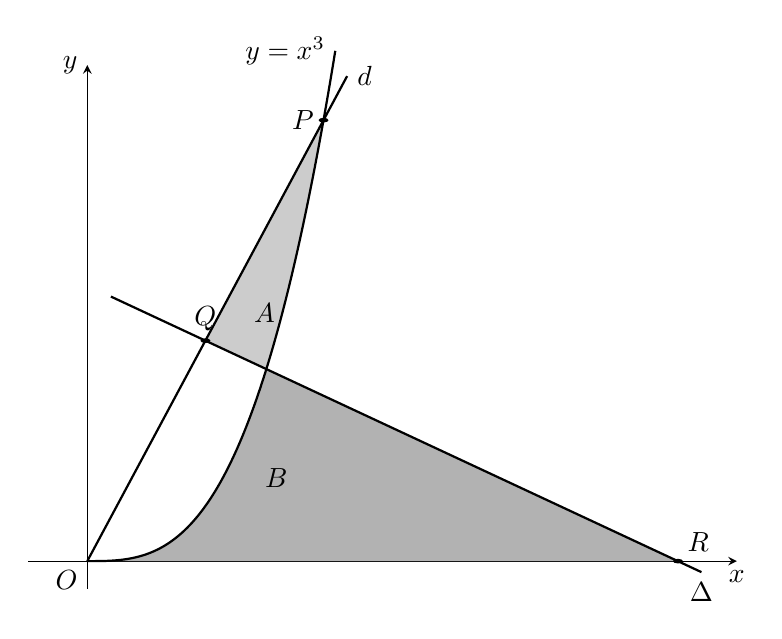
\begin{tikzpicture}[>=stealth, xscale=1.5, yscale=0.7]
		% Trục tọa độ
		\draw[->] (-0.5,0) -- (5.5,0) node[below] {$x$};
		\draw[->] (0,-0.5) -- (0,9) node[left] {$y$};
		\node[below left] at (0,0) {$O$};
		
		% Khai báo các tọa độ điểm mấu chốt
		\pgfmathsetmacro{\xP}{2}
		\pgfmathsetmacro{\yP}{8}
		\pgfmathsetmacro{\xQ}{1}
		\pgfmathsetmacro{\yQ}{4}
		\pgfmathsetmacro{\xR}{5}
		\pgfmathsetmacro{\yR}{0}
		
		% Điểm giao x_0 (nghiệm của x^3 = -x + 5)
		\pgfmathsetmacro{\xI}{1.51598}
		
		\coordinate (P) at (\xP, \yP);
		\coordinate (Q) at (\xQ, \yQ);
		\coordinate (R) at (\xR, \yR);
		\coordinate (O) at (0, 0);
		
		% Tô màu vùng A 
		\fill[gray!40] (Q) -- plot[domain=\xQ:\xI, smooth, variable=\x] (\x, {-\x+5}) -- plot[domain=\xI:\xP, smooth, variable=\x] (\x, {\x^3}) -- cycle;
		
		% Tô màu vùng B 
		\fill[gray!60] (O) -- plot[domain=0:\xI, smooth, variable=\x] (\x, {\x^3}) -- plot[domain=\xI:\xR, smooth, variable=\x] (\x, {-\x+5}) -- cycle;
		
		% Vẽ các đồ thị
		\draw[thick, smooth, samples=100, domain=0:2.1] plot (\x, {\x^3}) node[left] {$y=x^3$};
		\draw[thick, domain=0.2:5.2] plot (\x, {-\x+5}) node[below] {$\Delta$};
		\draw[thick, domain=0:2.2] plot (\x, {4*\x}) node[right] {$d$};
		
		% Các điểm và nhãn
		\fill (P) circle (1.2pt) node[left] {$P$};
		\fill (Q) circle (1.2pt) node[above] {$Q$};
		\fill (R) circle (1.2pt) node[above right] {$R$};
		
		% Nhãn A và B
		\node at (1.5, 4.5) {$A$};
		\node at (1.6, 1.5) {$B$};
		\end{tikzpicture}
	\end{center}
	
	\shortans{$6$}
	\loigiai{
		
		Ta có $f(2) = 2^3 = 8 \Rightarrow P(2; 8)$.
		Phương trình đường thẳng $d$ đi qua $O(0;0)$ và $P(2;8)$ là $y = 4x$.
		Hoành độ điểm $Q$ là nghiệm của phương trình hoành độ giao điểm giữa $d$ và $\Delta$: 
		$$4x = -x + 5 \Leftrightarrow 5x = 5 \Leftrightarrow x = 1 \Rightarrow Q(1; 4)$$
		Giao điểm $R$ của đường thẳng $\Delta: y = -x + 5$ với trục hoành là nghiệm của $-x + 5 = 0 \Leftrightarrow x = 5 \Rightarrow R(5; 0)$.
		
		Gọi $x_0$ là hoành độ giao điểm của đường cong $y=f(x)$ và đường thẳng $\Delta$. 
		Rõ ràng $x_0 \in (1; 2)$ vì đồ thị $f(x)$ cắt $\Delta$ ở giữa $x_Q$ và $x_P$. Phương trình $x^3 + x - 5 = 0$ có nghiệm vô tỉ $x_0 \approx 1,516$.
		Dựa vào đồ thị, ta có biểu thức tính diện tích các miền như sau:
		\begin{itemize}
			\item Miền $A$ được giới hạn phía trên bởi đoạn $PQ$ ($y=4x$), phía dưới bởi $\Delta$ (từ $x=1$ đến $x_0$) và $f(x)$ (từ $x_0$ đến $x=2$):
			$$A = \int_{1}^{x_0} \left[ 4x - (-x + 5) \right] \text{d}x + \int_{x_0}^{2} \left[ 4x - x^3 \right] \text{d}x$$
			\item Miền $B$ giới hạn bởi $f(x)$, $\Delta$ và trục hoành:
			$$B = \int_{0}^{x_0} x^3 \text{d}x + \int_{x_0}^{5} (-x + 5) \text{d}x$$
		\end{itemize}
		
		Xét hiệu $B - A$, ta thực hiện phép tính và nhóm các tích phân:
		\begin{align*}
		B - A &= \left[ \int_{0}^{x_0} x^3 \text{d}x + \int_{x_0}^{5} (-x + 5) \text{d}x \right] \\
		&\quad - \left[ \int_{1}^{x_0} 4x \text{d}x - \int_{1}^{x_0} (-x + 5) \text{d}x + \int_{x_0}^{2} 4x \text{d}x - \int_{x_0}^{2} x^3 \text{d}x \right] \\
		&= \left( \int_{0}^{x_0} x^3 \text{d}x + \int_{x_0}^{2} x^3 \text{d}x \right) + \left( \int_{x_0}^{5} (-x + 5) \text{d}x + \int_{1}^{x_0} (-x + 5) \text{d}x \right) \\
		&\quad - \left( \int_{1}^{x_0} 4x \text{d}x + \int_{x_0}^{2} 4x \text{d}x \right) \\
		&= \int_{0}^{2} x^3 \text{d}x + \int_{1}^{5} (-x + 5) \text{d}x - \int_{1}^{2} 4x \text{d}x
		\end{align*}
		
		Lúc này cận $x_0$ đã hoàn toàn bị triệt tiêu, ta tính 3 tích phân xác định đơn giản:
		\begin{itemize}
			\item $I_1 = \int_{0}^{2} x^3 \text{d}x = \frac{x^4}{4} \bigg|_{0}^{2} = 4$
			\item $I_2 = \int_{1}^{5} (-x + 5) \text{d}x = \left( -\frac{x^2}{2} + 5x \right) \bigg|_{1}^{5} = \frac{25}{2} - \frac{9}{2} = 8$
			\item $I_3 = \int_{1}^{2} 4x \text{d}x = 2x^2 \bigg|_{1}^{2} = 8 - 2 = 6$
		\end{itemize}
		Vậy $B - A = I_1 + I_2 - I_3 = 4 + 8 - 6 = 6$.
		
		\textbf{ĐS: } $\boldsymbol{6}$
	}
\end{ex}
\begin{ex}%[1H8H7-3]
	Cho hình chóp $S.ABCD$ có đáy là hình vuông cạnh $6$, $SA\perp ABCD$ và $SC=9$. Tính thể tích khối chóp $S.ABCD$.
	\begin{center}
		\begin{tikzpicture}[scale=0.7, font=\footnotesize,line join=round, line cap=round, >=stealth]
		\path 
		(0,0) coordinate (A)
		++(-140:2) coordinate (B)
		++(0:3.5) coordinate (C)
		($(A)+(C)-(B)$) coordinate (D)
		($(A)+(0,3)$) coordinate (S)
		;
		\foreach \i in{B,C,D}{\draw[blue] (S)--(\i);};
		\draw[blue] (B)--(C)--(D);
		\draw[blue, dashed] (S)--(A)--(B) (A)--(D);
		\pic[draw=blue,angle eccentricity=1.8,angle radius=2mm]{right angle=S--A--D};
		\foreach \i/\g in {A/-90,B/-90,C/-90,D/-90,S/90}
		\fill[blue] (\i) circle(1pt)+(\g:3mm)node[scale=1]{$\i$};
		\end{tikzpicture}
	\end{center}
	\shortans{$36$}
	\loigiai{
		\immini{Ta có $AC=\sqrt{6^2+6^2}=6\sqrt{2}$.\\
			Xét tam giác $SAC$ vuông tại $A$, ta có $SA=\sqrt{SC^2-AC^2}=\sqrt{9^2-(6\sqrt{2})^2}=3$.\\
			Khi đó $V_{S.ABCD}=\dfrac{1}{3}\cdot SA\cdot  AB^2=\dfrac{1}{3}\cdot 3\cdot 6^2=36$.}
		{\begin{tikzpicture}[scale=0.7, font=\footnotesize,line join=round, line cap=round, >=stealth]
			\path 
			(0,0) coordinate (A)
			++(-140:2) coordinate (B)
			++(0:3.5) coordinate (C)
			($(A)+(C)-(B)$) coordinate (D)
			($(A)+(0,3)$) coordinate (S)
			;
			\foreach \i in{B,C,D}{\draw[blue] (S)--(\i);};
			\draw[blue] (B)--(C)--(D);
			\draw[blue, dashed] (S)--(A)--(B) (A)--(D);
			\pic[draw=blue,angle eccentricity=1.8,angle radius=2mm]{right angle=S--A--D};
			\foreach \i/\g in {A/-90,B/-90,C/-90,D/-90,S/90}
			\fill[blue] (\i) circle(1pt)+(\g:3mm)node[scale=1]{$\i$};
			\end{tikzpicture}}
	}
\end{ex}

\begin{ex}%[2H5C2-8]
	Trong không gian với hệ trục tọa độ $Oxyz$, đơn vị trên mỗi trục toạ độ là mét, một thiết bị phát tia laser được đặt tại điểm $A(4;5;12)$. Thiết bị này chiếu một tia sáng về phía bức tường phẳng trùng với mặt phẳng tọa độ $(Oyz)$. Biết rằng tia sáng phát ra luôn thay đổi nhưng luôn tạo với trục $Ox$ một góc $45^\circ$. Gọi $M$ là vị trí vệt sáng laser chiếu lên bức tường. Khoảng cách lớn nhất từ vệt sáng $M$ đến gốc tọa độ $O$ bằng bao nhiêu mét?
	\shortans{$17$}
	\loigiai{
		\immini
		{
			Gọi $d$ là đường thẳng đi qua $A$ và vuông góc với mặt phẳng $(Oyz)$. Khi đó $d$ song song với trục $Ox$.\\
			Đường thẳng $d$ có phương trình: $\heva{& x=4+t \\ & y=5\\&z=12.}$\\
			Gọi $H$ là hình chiếu vuông góc của $A$ lên mặt phẳng $(Oyz) \Rightarrow H=d\cap (Oyz) \Rightarrow H(0;5;12)$.\\
			Ta có khoảng cách từ $A$ đến mặt tường $(Oyz)$ là $AH=4$.\\
			Do đường thẳng chứa tia laser $\Delta$ luôn tạo với $Ox$ (và dĩ nhiên tạo với $d$) một góc $45^\circ$, nên $\widehat{MAH}=45^\circ$.\\
			Xét tam giác $AHM$ vuông tại $H$, ta có:
			$$MH=AH\cdot \tan45^\circ = 4 \cdot 1 = 4 \ (\mathrm{m}).$$
			Suy ra tập hợp các vệt sáng $M$ trên tường là một đường tròn tâm $H(0;5;12)$, bán kính $R=4$ nằm trong mặt phẳng $(Oyz)$.\\
			Khoảng cách từ gốc tọa độ $O$ đến tâm $H$ là $OH = \sqrt{0^2 + 5^2 + 12^2} = 13 \ (\mathrm{m})$.\\
			Vệt sáng cách xa gốc tọa độ nhất khi $O, H, M$ thẳng hàng và $H$ nằm giữa $O$ và $M$. Khi đó, khoảng cách lớn nhất là:
			$$OM_{\mathrm{max}} = OH + R = 13 + 4 = 17 \ (\mathrm{m}).$$
		}
		{
			\begin{tikzpicture}[>=stealth,line join=round,line cap=round,font=\footnotesize,scale=.85, blue]
			\draw[->] (0,-.5) coordinate (O) node[below right]{$O$} -- (4.5,-.5) node[below]{$x$};
			\draw[->] (0,2) -- (0,4) node[right]{$z$};
			\draw[->] (0,-.5) -- (-3,-3) node[left]{$y$};
			\draw[dashed] (-2,3) arc(90:-90:.65cm and 2cm);
			\draw (-2,-1) arc(270:90:.65cm and 2cm);	
			\draw[dashed] (-2,1) coordinate (H) node[below left]{$H$} -- (2,1) coordinate (A) node[below]{$A$};
			\draw[dashed] (H) -- (-2,-1) coordinate (M') node[below]{$M'$};
			\coordinate (M) at ($(O)!1.32!(H)$);
			\coordinate (N) at ($(O)!0.16!(H)$);
			\fill (M) circle (1pt) node[left]{$M$};
			\fill (H) circle (1pt) (O) circle (1pt) (A) circle (1pt);
			\draw (N) -- (O) -- (0,0) (-2,3) -- (2,1) -- (-2,-1) (M) -- (A) -- ++(2,0) node[below left]{$d$};
			\draw (4,0) -- (A) -- ++(2,1) node[above left]{$\Delta$};
			\draw[dashed] (M) -- (N) (0,0) -- (0,2);
			\draw pic[draw=blue,fill=blue!15,angle radius=6mm,angle eccentricity=1.5,"$45^\circ$"] {angle = H--A--N};
			\draw pic[draw=blue,angle radius=2mm] {right angle = A--H--M'};
			\end{tikzpicture}
		}
	}
\end{ex}
\begin{ex}%[2D1V1-5]
	Một công ty công nghệ $A$ cung cấp nền tảng Trí tuệ nhân tạo dạng phần mềm dịch vụ cho các doanh nghiệp. Mỗi doanh nghiệp đăng ký sử dụng sẽ phải trả mức phí cố định là $50$ triệu đồng/năm. Tổng chi phí vận hành hệ thống máy chủ và bảo trì trong một năm mà công ty $A$ phải chi trả phụ thuộc vào số lượng doanh nghiệp $x$ ($x \in \mathbb{N}^*$) đang sử dụng phần mềm và được mô hình hóa bởi hàm số $C(x) = 100\ln(x) + 200$ (triệu đồng). Để công ty công nghệ $A$ đạt mức lợi nhuận tối thiểu là $5$ tỷ đồng trong một năm, công ty $A$ cần có ít nhất bao nhiêu doanh nghiệp sử dụng phần mềm đó?
	\shortans{$114$}
	\loigiai{
		Đổi $5$ tỷ đồng = $5000$ triệu đồng.\\
		Hàm doanh thu của công ty khi có $x$ khách hàng là: $F(x) = 50x$ (triệu đồng).\\
		Hàm lợi nhuận của công ty trong một năm là:
		$$P(x) = F(x) - C(x) = 50x - (100\ln x + 200) = 50x - 100\ln x - 200 \text{ (triệu đồng)}$$
		
		Để công ty đạt lợi nhuận tối thiểu là $5$ tỷ đồng thì $P(x) \ge 5000$. Ta có bất phương trình:
		\begin{align*}
		& 50x - 100\ln x - 200 \ge 5000 \\
		\Leftrightarrow\ & 50x - 100\ln x - 5200 \ge 0 \\
		\Leftrightarrow\ & x - 2\ln x - 104 \ge 0 \quad (*)
		\end{align*}
		
		Xét hàm số $g(x) = x - 2\ln x - 104$ trên tập xác định $D = [1; +\infty)$.\\
		Ta có đạo hàm: $g'(x) = 1 - \dfrac{2}{x} = \dfrac{x-2}{x}$.\\
		Cho $g'(x) = 0 \Leftrightarrow x = 2$.\\
		Với mọi $x \ge 3$, ta luôn có $g'(x) > 0$. Do đó, hàm số $g(x)$ đồng biến trên khoảng $(2; +\infty)$.
		
		Mặt khác, ta cần tìm số nguyên dương $x$ nhỏ nhất thỏa mãn bất phương trình $(*)$.\\
		Sử dụng chức năng TABLE trên máy tính cầm tay để dò nghiệm của phương trình $g(x)=0$ quanh giá trị $x \approx 100$, ta có:
		\begin{itemize}
			\item Tại $x = 113$: $g(113) = 113 - 2\ln(113) - 104 \approx -0{,}45 < 0$.
			\item Tại $x = 114$: $g(114) = 114 - 2\ln(114) - 104 \approx 0{,}52 > 0$.
		\end{itemize}
		Do hàm số $g(x)$ đồng biến và liên tục trên $(2; +\infty)$ nên $g(x) \ge 0 \Leftrightarrow x \ge 114$ (với $x \in \mathbb{N}^*$).\\
		
		Vậy công ty cần tìm kiếm ít nhất $114$ khách hàng doanh nghiệp trong năm đó để đạt được mục tiêu lợi nhuận đề ra.
	}
\end{ex}
\begin{ex}%[1D6H2-5]
	Đầu năm 2025, ông A thành lập một công ty. Tổng số tiền ông A dùng để trả lương cho nhân viên trong năm 2025 là $1$ tỷ đồng. Biết rằng cứ sau mỗi năm thì tổng số tiền dùng để trả lương cho nhân viên trong năm đó tăng thêm $15\%$ so với năm trước. Hỏi năm nào là năm đầu tiên mà tổng số tiền ông A dùng để trả lương cho nhân viên trong cả năm lớn hơn $2$ tỷ đồng?
	\shortans{$2030$}
	\loigiai{
		Gọi $n$ là số năm kể từ năm $2025$ ($n \in \mathbb{N}$).
		
		Tổng số tiền trả lương ở năm thứ $n$ (tức là năm $2025+n$) là: 
		$$1 \cdot (1 + 15\%)^n = 1,15^n \text{ (tỷ đồng)}$$
		
		Để tổng số tiền trả lương lớn hơn $2$ tỷ đồng, ta có bất phương trình:
		$$1,15^n > 2 \Leftrightarrow n > \log_{1,15}2 \approx 4,96$$
		
		Vì $n$ là số tự nhiên nên ta chọn $n = 5$.
		
		Vậy năm đầu tiên thỏa mãn yêu cầu bài toán là năm: $2025 + 5 = 2030$.
	}
\end{ex}

\Closesolutionfile{ans}

\indapan{6}{ans/ans-47-26-2-Cum7NB-L1-LC}
\indapan{4}{ans/ans-47-26-2-Cum7NB-L1-DS}
\indapan{6}{ans/ans-47-26-2-Cum7NB-L1-KQ}
